\documentclass[a4paper]{article}

\usepackage[margin=1in]{geometry}
\usepackage{amsmath}
\usepackage{amssymb}
\usepackage{graphicx}
\usepackage{float}
\usepackage{hyperref}
\usepackage{caption}
\usepackage{subcaption}
\usepackage{amsfonts}
\usepackage{pdfpages}
\usepackage[justification=centering]{caption}

\def\sectionautorefname{Section}
\def\subsectionautorefname{Section}
\def\subsubsectionautorefname{Section}
\def\figureautorefname{Figure}
\def\tableautorefname{Table}
\def\equationautorefname{Equation}


\begin{document}

%%%%%%%%%%%%%%%%%%%%%%%%%%
%%%%%%%%%%%%%%%%%%%%%%%%%%

\title{Random number generation}
\author{3F3 laboratory experiment \\ Theo A. Brown \\ Selwyn College, University of Cambridge}
\date{\today}
\maketitle

\tableofcontents

%%%%%%%%%%%%%%%%%%%%%%%%%%
%%%%%%%%%%%%%%%%%%%%%%%%%%

\section{Introduction}
Random numbers are widely used in science and engineering, forming the basis of stochastic modelling and
inference.
Generators of Gaussian and Uniform random numbers are widely implemented, but in many applications samples
from more complex distributions are required.
This report investigates methods for generating random numbers from different distributions.
Firstly, Uniform and Gaussian random number generators are used to investigate different methods for
estimating probability density functions (PDFs) from samples.
Secondly, samples from a new distribution are generated by transforming samples from a Uniform or
Gaussian distribution, using the Jacobian of the transformation.
Thirdly, Uniformly distributed random samples are transformed using the inverse cumulative density function
of the desired distribution.
Finally, samples from very complex distributions are generated using a scaled mixture of Gaussians, where
the desired distribution can be written as a Gaussian distribution with a random variance, set by some PDF.
In addition, Monte Carlo methods for estimating properties of a distribution from samples are investigated.

%%%%%%%%%%%%%%%%%%%%%%%%%%
%%%%%%%%%%%%%%%%%%%%%%%%%%

\section{Generating random numbers from the Uniform and Normal distributions}
\label{sec:uniform_normal}

A vector of 10000 samples from a unit Gaussian distribution was generated using \verb`np.random.randn`, and a vector of
10000 samples from a unit Uniform distribution was generated using \verb`np.random.rand`.
These sample vectors are used throughout the experiment to investigate different methods of random number generation.

%%%%%%%%%%%%%%%%%%%%%%%%%%

\subsection{Comparison of histogram with true probability density function}

The sample vectors were binned and plotted as histograms.
The true analytical probability density function (PDF) was calculated for the unit Gaussian and unit Uniform
distributions, and was overlaid on the histogram plots (\autoref{fig:histogram_and_pdf}).
It can be seen in \autoref{fig:histogram_and_pdf} that the histograms closely follow the shape of the analytical PDF,
showing that the generation of the random numbers for these distributions is accurate.

\begin{figure}[h]
    \centering
    \begin{subfigure}[b]{0.45\textwidth}
        \centering
        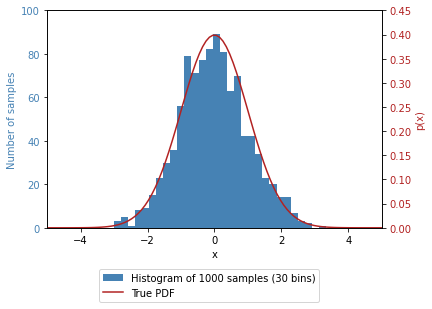
\includegraphics[width=\textwidth]{figures/gaussian_histogram_and_pdf.png}
        \caption{Gaussian distribution}
        \label{fig:gaussian_histogram_and_pdf}
    \end{subfigure}
    \hfill
    \begin{subfigure}[b]{0.45\textwidth}
        \centering
        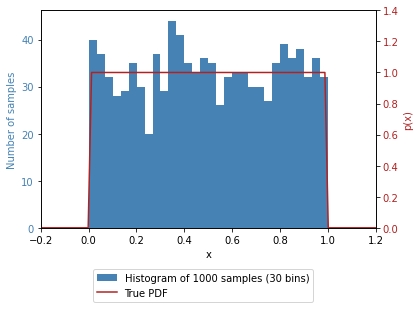
\includegraphics[width=\textwidth]{figures/uniform_histogram_and_pdf.png}
        \caption{Uniform distribution}
        \label{fig:uniform_histogram_and_pdf}
    \end{subfigure}
    \caption{Histogram of samples drawn from a distribution, overlaid with the true PDF of the distribution}
    \label{fig:histogram_and_pdf}
\end{figure}

%%%%%%%%%%%%%%%%%%%%%%%%%%

\subsection{Kernel density smoothing}

A unit Gaussian kernel $\mathcal{N}(0, 1)$ is applied to the data to provide a continuous estimate for the PDF.
The result is plotted for the Gaussian and Uniform distributions in \autoref{fig:kernel_smoothed}.

\begin{figure}[h]
    \centering
    \begin{subfigure}[b]{0.45\textwidth}
        \centering
        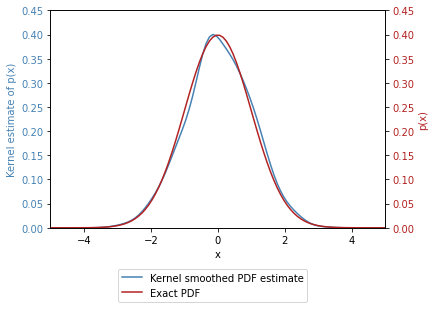
\includegraphics[width=\textwidth]{figures/gaussian_kernel_smoothed.png}
        \caption{Gaussian distribution}
        \label{fig:gaussian_kernel_smoothed}
    \end{subfigure}
    \hfill
    \begin{subfigure}[b]{0.45\textwidth}
        \centering
        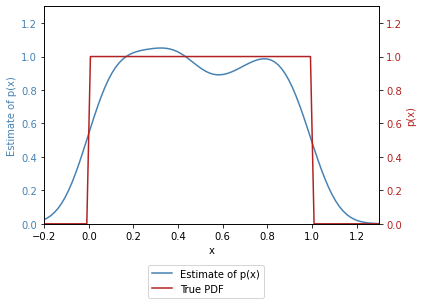
\includegraphics[width=\textwidth]{figures/uniform_kernel_smoothed.png}
        \caption{Uniform distribution}
        \label{fig:uniform_kernel_smoothed}
    \end{subfigure}
    \caption{Estimate of the PDF of a distribution, generated using Gaussian kernel smoothing of random samples from the
             distribution, overlaid with the true PDF of the distribution}
    \label{fig:kernel_smoothed}
\end{figure}

At each point, the kernel method takes the mean of N neighbouring values, weighted using a Gaussian distribution.
This is advantageous as it can smooth random irregularities in the samples: for example, there may be histogram bins
with a sample count that is greater than the expected sample count, which would give an incorrectly high estimate of
the probability of a sample falling in this bin; the kernel smooths out this local peak by taking neighbouring values
into account.
However, this also means that the kernel smoothing method becomes inaccurate when there is a sudden change or
discontinuity in the probability density function.
In the Uniform distribution there is zero probability for values outside the range $0<x<1$, but as the kernel averages
over a window of values it does not capture the step change at $x=0$ and $x=1$ and instead decays smoothly.

%%%%%%%%%%%%%%%%%%%%%%%%%%

\subsection{Multinomial distribution theory}

\subsubsection{Derivation of the multinomial distribution}
For $N$ samples and $M$ bins, let $N_i$ be the random variable representing the number of samples in bin $i$ and $p_i$
be the probability that a sample falls in bin $i$.
Samples are drawn independently, so the probability of getting $n_i$ samples in bin $i$ is given by:
\begin{align*}
    Pr(N_i = n_i) = \prod_{j=1}^{n_i} p_i = p_i^{n_i}
\end{align*}
The joint probability of obtaining a given distribution of $N$ samples across $M$ bins is given by:
\begin{align}
    \label{eq:joint_bin_probability_1}
    Pr(N_1 = n_1, N_2 = n_2, \dots, N_M= n_M) =
     \prod_{i=1}^{M} {N_{\text{available}, i} \choose {n_i}} p_i^{n_i}
\end{align}
where $N_{\text{available}, i} = N - \sum_{j=1}^{i-1} n_j$.

The binomial coefficient in \autoref{eq:joint_bin_probability_1} comes from considering all possible combinations of
getting $n_i$ samples in bin $i$:
\begin{itemize}
    \item For the first bin, $n_1$ samples are chosen from a set of $N$
    \item For the second bin, $n_2$ samples are chosen from a set of $N - n_1$
    \item For the $i$th bin, $n_i$ samples are chosen from a set of $N - n_1 \dots - n_{i-1}$
\end{itemize}
Simplifying the coefficient in \autoref{eq:joint_bin_probability_1} gives:
\begin{align*}
    {N \choose n_1}{N - n_1 \choose n_2} \dots {n_M \choose n_M}
  & = \frac{N!}{n_1!(N - n_1)!} \frac{(N - n_1)!}{n_2!(N - n_1 - n_2)!} \dots \frac{n_M!}{n_M!} \\
  & = \frac{N!}{n_1! n_2! \dots n_M!}
\end{align*}
The last step above is obtained by diagonal cancellation.

Consequently, \autoref{eq:joint_bin_probability_1} simplifies to:
\begin{align*}
    Pr(N_1 = n_1, N_2 = n_2, \dots, N_M = n_M) = \frac{N!}{n_1! n_2! \dots n_M!} p_1^{n_1} p_2^{n_2} ... p_M^{n_M}
\end{align*}

From considering the probability $p_i = Pr(N_i = n_i)$ for $N$ samples, the mean and standard deviation of $N_i$ can be
found:
\begin{align}
    \label{eq:bin_mean}
    \mu_i &= \mathbb{E}[N_i] = N p_i \\
    \label{eq:bin_sd}
    \sigma_i &= \sqrt{Var[N_i]} = \sqrt{N p_i (1 - p_i)}
\end{align}

%%%%%%%%%%%%%%%%%%%%%%%%%%

\subsubsection{Application to the Uniform distribution}
For the Uniform distribution between 0 and 1, the pdf $p(x)$ is defined as:
\begin{align*}
    p(x) &= \frac{1}{x_{max} - x_{min}} \\
         &= 1
\end{align*}
Hence, using \autoref{eq:bin_mean} and \autoref{eq:bin_sd}, the mean and standard deviation of the number of samples from the
Uniform distribution in a histogram with bin width $\delta$ and bin centers $c_i$:
\begin{align*}
    p_i &= \int_{c_i - \delta/2}^{c_i + \delta/2}1\,dx \\
        &= \delta \\
    \mu_i &= N \delta \\
    \sigma_i &= \sqrt{N \delta (1 - \delta)}
\end{align*}

\begin{figure}[h]
    \centering
    \begin{subfigure}[b]{0.3\textwidth}
        \centering
        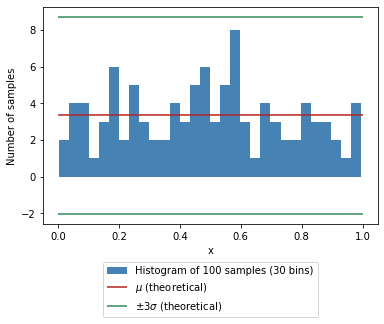
\includegraphics[width=\textwidth]{figures/uniform_histogram_100.png}
        \caption{$N=100$}
        \label{fig:uniform_histogram_100}
    \end{subfigure}
    \hfill
    \begin{subfigure}[b]{0.3\textwidth}
        \centering
        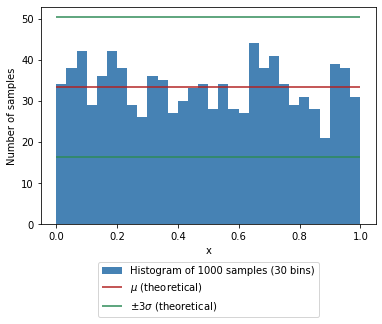
\includegraphics[width=\textwidth]{figures/uniform_histogram_1000.png}
        \caption{$N=1000$}
        \label{fig:uniform_histogram_1000}
    \end{subfigure}
    \hfill
    \begin{subfigure}[b]{0.3\textwidth}
        \centering
        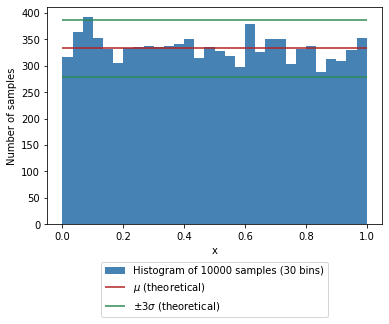
\includegraphics[width=\textwidth]{figures/uniform_histogram_10000.png}
        \caption{$N=10000$}
        \label{fig:uniform_histogram_10000}
    \end{subfigure}
    \caption{Histogram of N samples from a Uniform distribution, showing mean and $\pm3$ standard deviation}
    \label{fig:uniform_histogram_increasing_N}
\end{figure}

\autoref{fig:uniform_histogram_increasing_N} shows that the sample count lies within the $3\sigma$ interval for almost
all bins, which is consistent with the multinomial distribution theory.

%%%%%%%%%%%%%%%%%%%%%%%%%%

\subsubsection{Application to the Gaussian distribution}

\begin{figure}[h]
    \centering
    \begin{subfigure}[b]{0.3\textwidth}
        \centering
        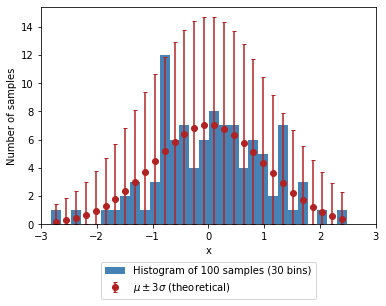
\includegraphics[width=\textwidth]{figures/gaussian_histogram_100.png}
        \caption{$N=100$}
        \label{fig:gaussian_histogram_100}
    \end{subfigure}
    \hfill
    \begin{subfigure}[b]{0.3\textwidth}
        \centering
        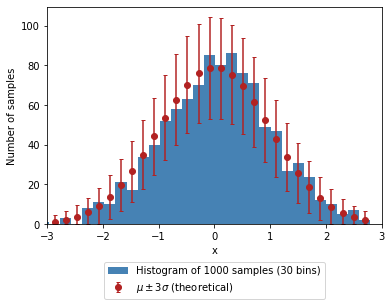
\includegraphics[width=\textwidth]{figures/gaussian_histogram_1000.png}
        \caption{$N=1000$}
        \label{fig:gaussian_histogram_1000}
    \end{subfigure}
    \hfill
    \begin{subfigure}[b]{0.3\textwidth}
        \centering
        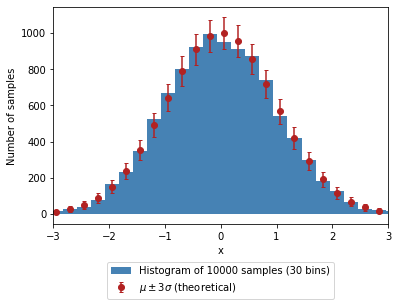
\includegraphics[width=\textwidth]{figures/gaussian_histogram_10000.png}
        \caption{$N=10000$}
        \label{fig:gaussian_histogram_10000}
    \end{subfigure}
    \caption{Histogram of N samples from a Gaussian distribution, showing mean and $\pm3$ standard deviation}
    \label{fig:gaussian_histogram_increasing_N}
\end{figure}

\autoref{fig:gaussian_histogram_increasing_N} shows that the sample count lies within the $3\sigma$ interval for almost
all bins, which is consistent with the multinomial distribution theory.

%%%%%%%%%%%%%%%%%%%%%%%%%%

\subsubsection{Effect of increasing $N$}
Multinomial distribution theory suggests that the method of using a histogram of samples to estimate properties of a
distribution increases in accuracy as the number of samples $N$ increases.
For a given bin probability $p_j$, the standard deviation increases less rapidly than the mean with increasing $N$
($\sigma \propto \sqrt{N}$ whereas $\mu \propto N$).
Consequently an increase in $N$ will result in the standard deviation becoming smaller compared to the mean
($\frac{\sigma}{\mu} \propto \frac{1}{\sqrt{N}}$).
This can be seen in \autoref{fig:uniform_histogram_increasing_N} and \autoref{fig:gaussian_histogram_increasing_N},
where the standard deviation reduces as $N$ increases.

%%%%%%%%%%%%%%%%%%%%%%%%%%

\subsubsection{Effect of bin probabilities}
\autoref{fig:gaussian_histogram_increasing_N} shows that the variance in the number of samples $N_i$ in bin $i$
increases as $p_i$ increases.
\autoref{eq:bin_sd} demonstrates the relationship between $Var[N_i]$ and $p_i$.
For $p_i$ close to zero,


%%%%%%%%%%%%%%%%%%%%%%%%%%
%%%%%%%%%%%%%%%%%%%%%%%%%%

\section{Functions of random variables}

\subsection{$f = a x + b$}
For $x \sim \mathcal{N}(0, 1)$, let $y = f(x) = a x + b$. Then:
\begin{align*}
    f^{-1}(y) &= \frac{y - b}{a} \\
    \left|\frac{dy}{dx}\right| &= |a| \\
    p_Y(y) &= \frac{1}{|a|} p_X \left( \frac{y - b}{a} \right) \\
    &= \frac{1}{|a|}\times\frac{1}{\sqrt{2\pi}} \exp{\left( -\frac{1}{2} \left( \frac{y-b}{a} \right)^2 \right)}
\end{align*}
Comparing with the equation for a general Gaussian distribution, it is clear that $p_Y(y)$ is a Gaussian distribution
with mean $b$ and variance $a^2$. This is shown in \autoref{fig:linear_function_of_gaussian}.

\begin{figure}[h]
    \centering
    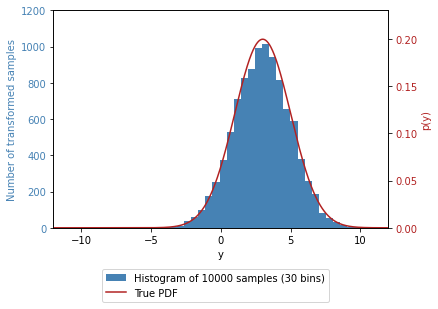
\includegraphics[width=0.6\textwidth]{figures/linear_function_of_gaussian.png}
    \caption{Histogram of linear function ($f(x^{(i)}) = 2x^{(i)} + 3$) of Gaussian samples overlaid with
    calculated PDF}
    \label{fig:linear_function_of_gaussian}
\end{figure}

%%%%%%%%%%%%%%%%%%%%%%%%%%

\subsection{$f = x^2$}
For $x \sim \mathcal{N}(0, 1)$, let $y = f(x) = x ^ 2$. Then:
\begin{align*}
    f^{-1}(y) &= \pm \sqrt{y} \\
    \left|\frac{dy}{dx}\right| &= |2x| \\
    p_Y(y) &= \sum_{i=1}^{2} \frac{1}{|2 \sqrt{y}|} p_X \left( \sqrt{y} \right) \\
    &= \frac{1}{\sqrt{2\pi y}} \exp{\left( -\frac{1}{2} y \right)}
\end{align*}

The result is plotted in \autoref{fig:quadratic_function_of_gaussian}.

\begin{figure}[h]
\centering
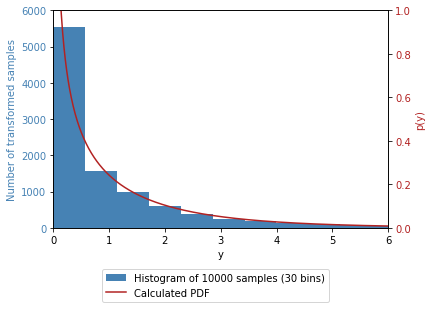
\includegraphics[width=0.6\textwidth]{figures/quadratic_function_of_gaussian.png}
\caption{Histogram of quadratic function $\left(f(x^{(i)}) = \left(x^{(i)}\right)^2\right)$) of Gaussian samples
overlaid with calculated PDF}
\label{fig:quadratic_function_of_gaussian}
\end{figure}

%%%%%%%%%%%%%%%%%%%%%%%%%%
%%%%%%%%%%%%%%%%%%%%%%%%%%

\section{Generating random variables using the inverse CDF method}

For the exponential distribution with mean one:
\begin{align*}
    & \text{PDF: } p(y) = \exp(-y), \ y \geq 0 \\
    & \text{CDF: } F(y) = \int_0^y p(y') dy' = 1 - \exp(-y) \\
    & \text{iCDF: } F^{-1}(x) = -\ln(1 - x)
\end{align*}

\autoref{fig:icdf_exponential} shows that samples from the exponential distribution generated using the iCDF follow the
true PDF.

\begin{figure}[h]
\centering
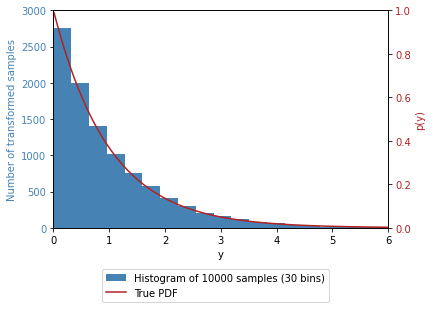
\includegraphics[width=0.6\textwidth]{figures/icdf_exponential.png}
\caption{Histogram of samples drawn from the uniform distribution and transformed using the iCDF method to follow the
exponential distribution, overlaid with the true exponential PDF}
\label{fig:icdf_exponential}
\end{figure}


%%%%%%%%%%%%%%%%%%%%%%%%%%
%%%%%%%%%%%%%%%%%%%%%%%%%%

\section{Simulation from non-standard densities}

Using the iCDF method, we can generate samples that are distributed according to:
\begin{align*}
    p(u) = \frac{\alpha^2}{2} \exp\left(-\frac{\alpha^2}{2} u\right)
\end{align*}
This distribution has:
\begin{align*}
    & \text{CDF: } F(u) = \int_0^u p(u') du' = 1 - \exp\left(-\frac{\alpha^2}{2} u\right) \\
    & \text{iCDF: } F^{-1}(v) = -\frac{2}{\alpha^2} \ln(1 - v)
\end{align*}
Samples $u^{(i)}$ can therefore be generated from uniformly distributed samples $v^(i)$.
The samples $u^{(i)}$ are then used to set the variance of the random variable X:
\begin{align*}
    p(x) = int_{0}^{\inf} \mathcal{N}(x\,|0, u) p(u) du
\end{align*}
The limit of the integral is from zero to infinity because the standard deviation must be positive.
A histogram of samples of $x^{(i)}$ is plotted in \autoref{fig:nonstandard_distribution} for different values of
$\alpha$. It appears that $\alpha$ sets the standard deviation of the distribution.
\begin{figure}[h]
\centering
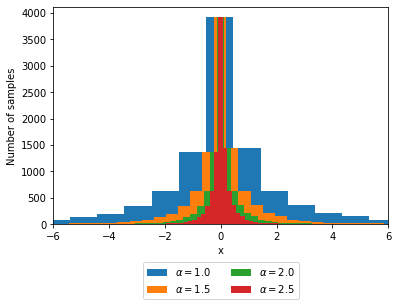
\includegraphics[width=0.6\textwidth]{figures/nonstandard_distribution.png}
\caption{100-bin histogram of samples drawn from the example distribution for different values of $\alpha$}
\label{fig:nonstandard_distribution}
\end{figure}

The kernel method was applied to the data, and the smoothed density was plotted on linear and log axes at different
scales (\autoref{fig:nonstandard_distribution_kernel_smoothed}). From the shape of the distribution
seems to be a sharper version of a Gaussian distribution, with significantly higher probability density in the centre
and tails that last for longer. Closer examination of the logarithmic plots suggests that the distribution behaves
more like a Gaussian close to $x=0$, where the logarithmic graph resembles an inverted parabola, and more like an
exponential further from $x=0$, where the logarithmic graph becomes linear.


\begin{figure}[h]
    \centering
    \begin{subfigure}[b]{0.3\textwidth}
        \centering
        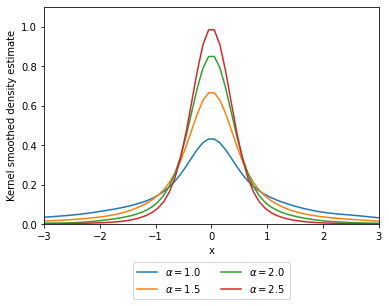
\includegraphics[width=\textwidth]{figures/nonstandard_distribution_ksdensity.png}
        \caption{Linear scale}
        \label{fig:nonstandard_distribution_kernel_smoothed_linear}
    \end{subfigure}
    \hfill
    \begin{subfigure}[b]{0.3\textwidth}
        \centering
        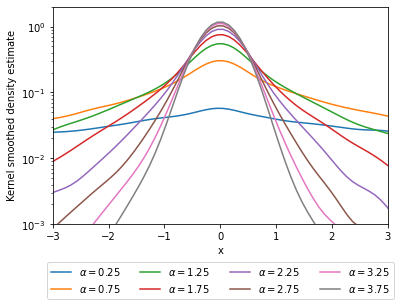
\includegraphics[width=\textwidth]{figures/nonstandard_distribution_ksdensity_log_close.png}
        \caption{$10^{-3} < \ln(p(x)) < 1$}
        \label{fig:nonstandard_distribution_ksdensity_log_close}
    \end{subfigure}
    \hfill
    \begin{subfigure}[b]{0.3\textwidth}
        \centering
        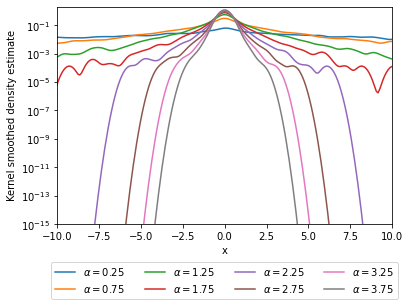
\includegraphics[width=\textwidth]{figures/nonstandard_distribution_ksdensity_log_far.png}
        \caption{$10^{-15} < \ln(p(x)) < 1$}
        \label{fig:nonstandard_distribution_ksdensity_log_far}
    \end{subfigure}
    \caption{Kernel smoothed probability density estimates for the example distribution}
    \label{fig:nonstandard_distribution_kernel_smoothed}
\end{figure}

%%%%%%%%%%%%%%%%%%%%%%%%%%
%%%%%%%%%%%%%%%%%%%%%%%%%%

\newpage
%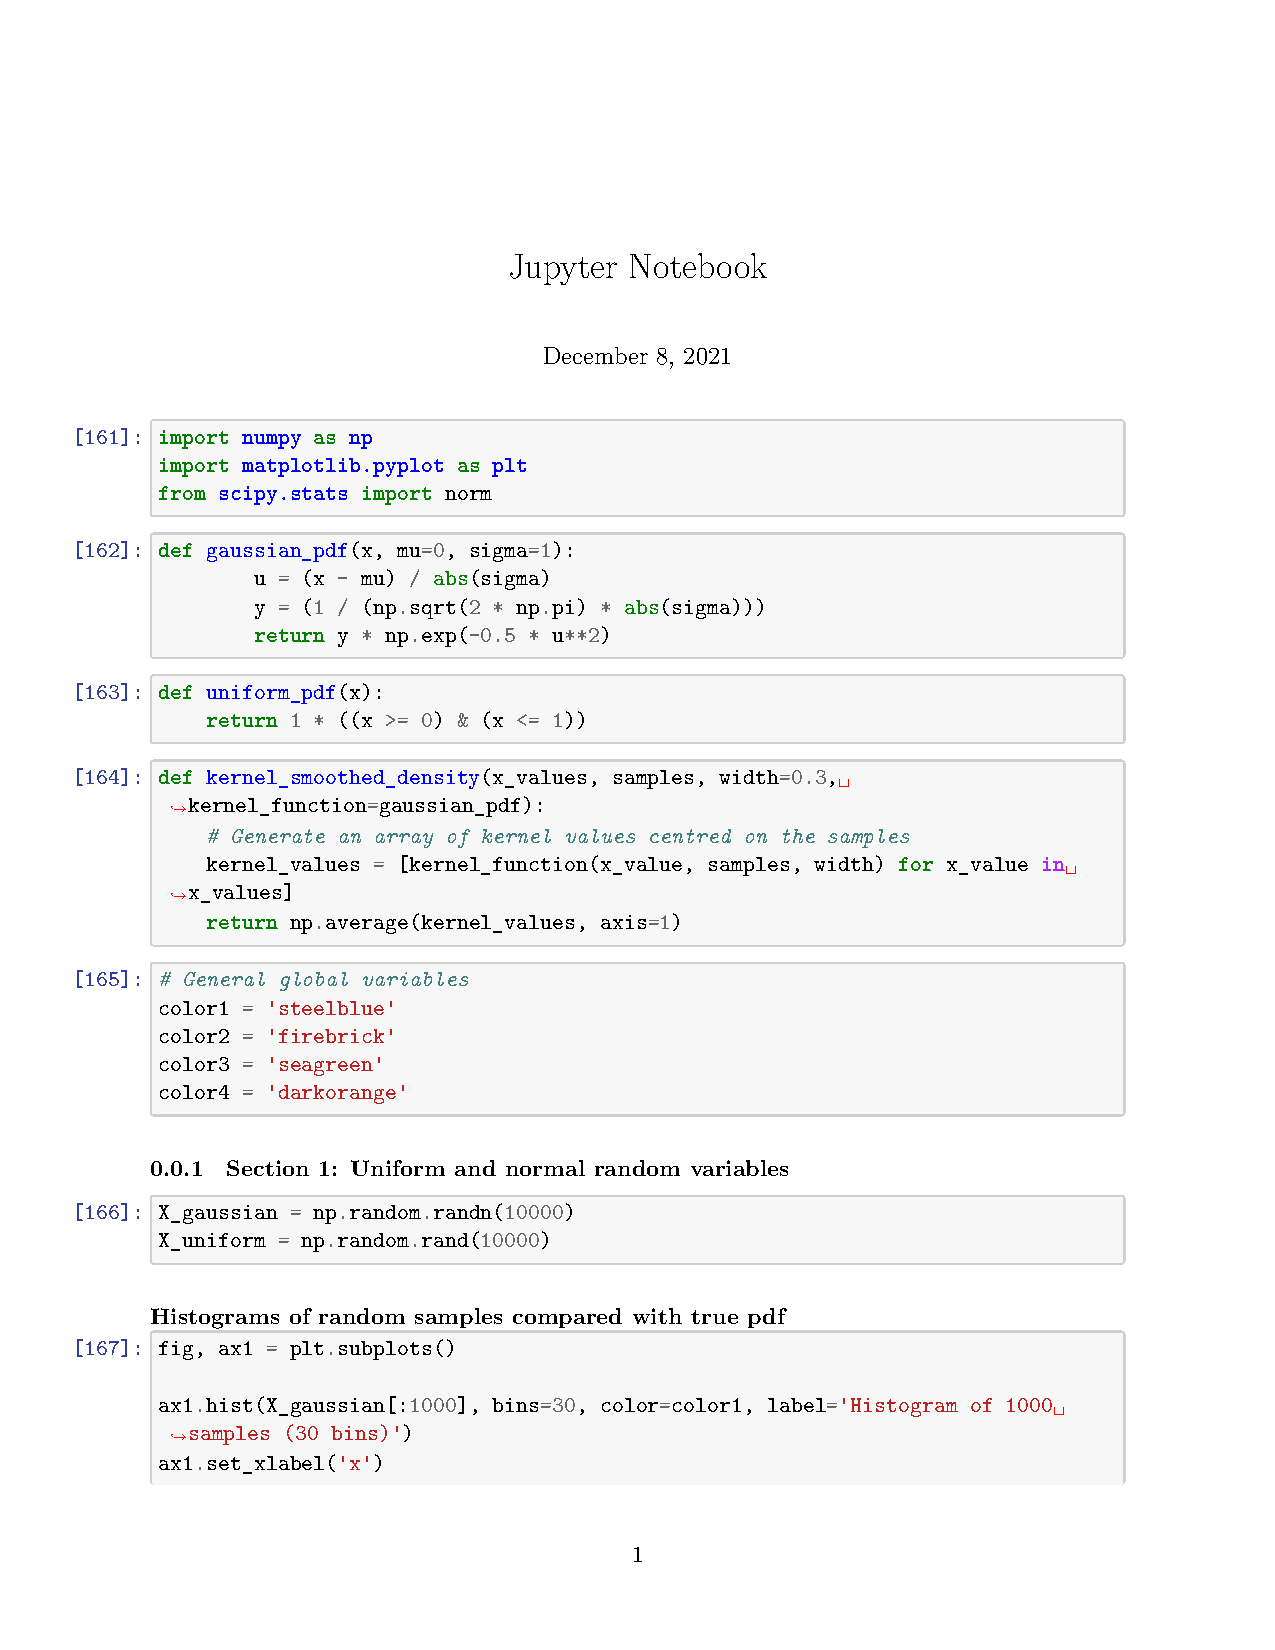
\includepdf[pages=-]{out/Jupyter Notebook.pdf}

\end{document}